\documentclass[aspectratio=169]{beamer}
% Loading required packages
\usepackage[utf8]{inputenc}
\usepackage{hyperref}
\usepackage{tikz}
\usepackage{fontawesome5}
\usepackage{xcolor}
\usepackage{graphicx}
\usepackage{adjustbox}

% Defining Google Colors
\definecolor{googleblue}{HTML}{4285F4}
\definecolor{googlered}{HTML}{EA4335}
\definecolor{googleyellow}{HTML}{FBBC04}
\definecolor{googlegreen}{HTML}{34A853}
\definecolor{darkgray}{HTML}{5F6368}

% Configuring Beamer theme
\usetheme{Madrid}
\usecolortheme{default}

% Setting up color theme
\setbeamercolor{palette primary}{bg=googleblue,fg=white}
\setbeamercolor{palette secondary}{bg=googleblue!80,fg=white}
\setbeamercolor{palette tertiary}{bg=googleblue!60,fg=white}
\setbeamercolor{structure}{fg=googleblue}
\setbeamercolor{title}{fg=googleblue}
\setbeamercolor{frametitle}{bg=googleblue,fg=white}
\setbeamercolor{block title}{bg=googleblue,fg=white}
\setbeamercolor{block body}{bg=gray!10}
\setbeamercolor{item}{fg=googleblue}
\setbeamercolor{subitem}{fg=googlegreen}
\setbeamercolor{subsubitem}{fg=googlered}

% Removing navigation symbols
\setbeamertemplate{navigation symbols}{}

% Creating custom header
\setbeamertemplate{headline}{%
    \begin{beamercolorbox}[wd=\paperwidth,ht=2.5ex,dp=1ex,center]{palette primary}
        \insertframenumber/\inserttotalframenumber \hfill \insertsectionhead
    \end{beamercolorbox}
}

% Creating custom footer
\setbeamertemplate{footline}{%
    \begin{beamercolorbox}[wd=\paperwidth,ht=3ex,dp=1.5ex,center]{palette primary}
        \begin{minipage}[c]{0.33\paperwidth}
            \scriptsize\color{white}
            \hfill \href{https://easy-ai-labs.lovable.app/}{\color{white}\faIcon{globe} Easy AI Labs}
        \end{minipage}%
        \begin{minipage}[c]{0.33\paperwidth}
            \centering
            \scriptsize\color{white}
            \href{https://www.linkedin.com/in/yashkavaiya}{\color{white}\faIcon{linkedin} Yash Kavaiya}
        \end{minipage}%
        \begin{minipage}[c]{0.33\paperwidth}
            \scriptsize\color{white}
            \href{https://www.linkedin.com/company/genai-guru}{\color{white}\faIcon{building} Gen AI Guru} \hfill
        \end{minipage}
    \end{beamercolorbox}
}

% Setting title and author information
\title[Marriage Compatibility App]{\textbf{Marriage Compatibility Assessment Platform}}
\subtitle{Building Stronger Relationships Through AI-Powered Analysis}
\author[Yash Kavaiya]{Presented by: Yash Kavaiya}
\institute[Gen AI Guru]{
    \textbf{Gen AI Guru} \\
    \small AI Solutions for Modern Relationships
}
\date{\today}

\begin{document}

% Creating title slide
{
\setbeamertemplate{headline}{}
\setbeamertemplate{footline}{}
\begin{frame}
    \begin{tikzpicture}[remember picture,overlay]
        \fill[googleblue!10] (current page.south west) rectangle (current page.north east);
        \fill[googleblue] (current page.north west) rectangle ([xshift=3cm]current page.south west);
        \fill[googlered] ([xshift=3cm]current page.north west) rectangle ([xshift=3.3cm]current page.south west);
        \fill[googleyellow] ([xshift=3.3cm]current page.north west) rectangle ([xshift=3.6cm]current page.south west);
        \fill[googlegreen] ([xshift=3.6cm]current page.north west) rectangle ([xshift=3.9cm]current page.south west);
    \end{tikzpicture}
    
    \vspace{0.5cm}
    \begin{center}
        {\Huge \color{googleblue}\textbf{Marriage Compatibility}}\\
        \vspace{0.2cm}
        {\LARGE \color{googlered}\textbf{Assessment Platform}}\\
        \vspace{0.8cm}
        {\large \color{darkgray}\textit{Empowering Couples with AI-Driven Insights}}\\
        \vspace{1cm}
        
        \begin{minipage}{0.7\textwidth}
            \centering
            \begin{beamercolorbox}[wd=\textwidth,sep=8pt,center,rounded=true,shadow=true]{palette primary}
                \color{white}
                \textbf{86 Questions} • \textbf{14 Life Areas} • \textbf{Smart Analytics}
            \end{beamercolorbox}
        \end{minipage}
        
        \vspace{0.8cm}
        {\normalsize 
            \href{https://easy-ai-labs.lovable.app/}{\color{googleblue}\faIcon{globe} easy-ai-labs.lovable.app} \\
            \vspace{0.2cm}
            Presented by: \textbf{Yash Kavaiya}
        }
    \end{center}
\end{frame}
}

% Creating overview slide
\section{Platform Overview}
\begin{frame}{Platform Overview}
    \begin{columns}[T]
        \column{0.48\textwidth}
        \begin{block}{What We Built}
            \begin{itemize}
                \item React-based web application
                \item TypeScript for type safety
                \item Tailwind CSS for styling
                \item PDF report generation
                \item Voice assessment capability
            \end{itemize}
        \end{block}
        
        \column{0.48\textwidth}
        \begin{center}
            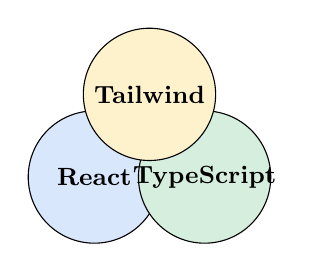
\begin{tikzpicture}[scale=0.7]
                \draw[fill=googleblue!20] (0,0) circle (1.2cm);
                \draw[fill=googlegreen!20] (2,0) circle (1.2cm);
                \draw[fill=googleyellow!20] (1,1.5) circle (1.2cm);
                \node at (0,0) {\small\textbf{React}};
                \node at (2,0) {\small\textbf{TypeScript}};
                \node at (1,1.5) {\small\textbf{Tailwind}};
            \end{tikzpicture}
            \vspace{0.3cm}
            \begin{alertblock}{Key Innovation}
                AI-powered voice assessment using speech recognition
            \end{alertblock}
        \end{center}
    \end{columns}
\end{frame}

% Creating key features slide
\section{Key Features}
\begin{frame}{Key Features}
    \begin{columns}[T]
        \column{0.33\textwidth}
        \begin{center}
            \tikz\draw[fill=googleblue!30,draw=googleblue,thick] (0,0) circle (0.8cm);
            \vspace{0.2cm}
            {\color{googleblue}\Large\faIcon{question-circle}}\\
            \vspace{0.2cm}
            \textbf{86 Questions}\\
            \small Comprehensive assessment covering all aspects
        \end{center}
        
        \column{0.33\textwidth}
        \begin{center}
            \tikz\draw[fill=googlegreen!30,draw=googlegreen,thick] (0,0) circle (0.8cm);
            \vspace{0.2cm}
            {\color{googlegreen}\Large\faIcon{chart-pie}}\\
            \vspace{0.2cm}
            \textbf{14 Categories}\\
            \small From values to lifestyle choices
        \end{center}
        
        \column{0.33\textwidth}
        \begin{center}
            \tikz\draw[fill=googlered!30,draw=googlered,thick] (0,0) circle (0.8cm);
            \vspace{0.2cm}
            {\color{googlered}\Large\faIcon{file-pdf}}\\
            \vspace{0.2cm}
            \textbf{PDF Reports}\\
            \small Detailed compatibility analysis
        \end{center}
    \end{columns}
    
    \vspace{0.4cm}
    \begin{beamercolorbox}[wd=0.9\textwidth,sep=5pt,center,rounded=true]{palette secondary}
        \color{white}\textbf{Dual Rating System:} Importance (1-5) + Flexibility (1-5)
    \end{beamercolorbox}
\end{frame}

% Creating assessment categories slide
\section{Assessment Categories}
\begin{frame}{14 Life Assessment Categories}
    \begin{columns}[T]
        \column{0.48\textwidth}
        \begin{enumerate}
            \item \textcolor{googleblue}{Core Values \& Ethics}
            \item \textcolor{googlegreen}{Religion}
            \item \textcolor{googlered}{Spirituality}
            \item \textcolor{googleyellow}{Relationship Model}
            \item \textcolor{googleblue}{Life Vision \& Home}
            \item \textcolor{googlegreen}{Children \& Parenting}
            \item \textcolor{googlered}{Finances}
        \end{enumerate}
        
        \column{0.48\textwidth}
        \begin{enumerate}
            \setcounter{enumi}{7}
            \item \textcolor{googleyellow}{Work \& Career}
            \item \textcolor{googleblue}{Household \& Roles}
            \item \textcolor{googlegreen}{Communication}
            \item \textcolor{googlered}{Love \& Intimacy}
            \item \textcolor{googleyellow}{Health \& Lifestyle}
            \item \textcolor{googleblue}{Family \& In-Laws}
            \item \textcolor{googlegreen}{Growth \& Change}
        \end{enumerate}
    \end{columns}
    
    \vspace{0.4cm}
    \begin{alertblock}{Comprehensive Coverage}
        Each category contains multiple questions targeting specific relationship aspects
    \end{alertblock}
\end{frame}

% Creating technology stack slide
\section{Technology Stack}
\begin{frame}{Technology Stack}
    \begin{center}
        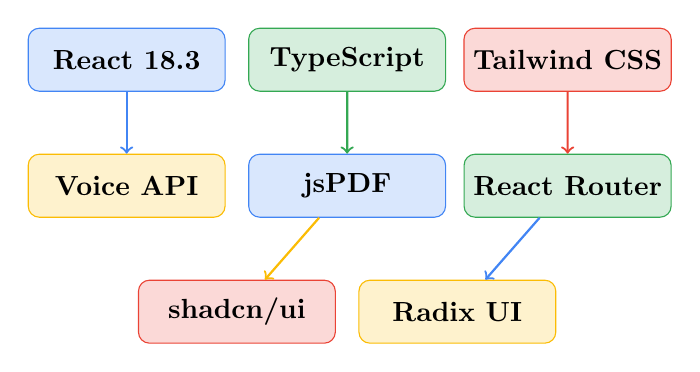
\begin{tikzpicture}[scale=0.8]
            \node[draw=googleblue,fill=googleblue!20,rounded corners,minimum width=2.5cm,minimum height=0.8cm] (react) at (0,3) {\textbf{React 18.3}};
            \node[draw=googlegreen,fill=googlegreen!20,rounded corners,minimum width=2.5cm,minimum height=0.8cm] (ts) at (3.5,3) {\textbf{TypeScript}};
            \node[draw=googlered,fill=googlered!20,rounded corners,minimum width=2.5cm,minimum height=0.8cm] (tailwind) at (7,3) {\textbf{Tailwind CSS}};
            
            \node[draw=googleyellow,fill=googleyellow!20,rounded corners,minimum width=2.5cm,minimum height=0.8cm] (voice) at (0,1) {\textbf{Voice API}};
            \node[draw=googleblue,fill=googleblue!20,rounded corners,minimum width=2.5cm,minimum height=0.8cm] (pdf) at (3.5,1) {\textbf{jsPDF}};
            \node[draw=googlegreen,fill=googlegreen!20,rounded corners,minimum width=2.5cm,minimum height=0.8cm] (routing) at (7,1) {\textbf{React Router}};
            
            \node[draw=googlered,fill=googlered!20,rounded corners,minimum width=2.5cm,minimum height=0.8cm] (shadcn) at (1.75,-1) {\textbf{shadcn/ui}};
            \node[draw=googleyellow,fill=googleyellow!20,rounded corners,minimum width=2.5cm,minimum height=0.8cm] (radix) at (5.25,-1) {\textbf{Radix UI}};
            
            \draw[->,thick,googleblue] (react) -- (voice);
            \draw[->,thick,googlegreen] (ts) -- (pdf);
            \draw[->,thick,googlered] (tailwind) -- (routing);
            \draw[->,thick,googleyellow] (pdf) -- (shadcn);
            \draw[->,thick,googleblue] (routing) -- (radix);
        \end{tikzpicture}
    \end{center}
    
    \vspace{0.3cm}
    \begin{beamercolorbox}[wd=0.9\textwidth,sep=5pt,center,rounded=true]{palette primary}
        \color{white}\textbf{Build Tool:} Vite 5.4 • \textbf{Package Manager:} npm
    \end{beamercolorbox}
\end{frame}

% Creating user experience flow slide
\section{User Experience}
\begin{frame}{User Experience Flow}
    \begin{tikzpicture}[
        node distance=1.8cm,
        block/.style={rectangle, draw, fill=googleblue!20, text width=2.2cm, text centered, rounded corners, minimum height=0.7cm},
        decision/.style={diamond, draw, fill=googleyellow!20, text width=1.8cm, text centered, minimum height=0.7cm, aspect=1.5},
        arrow/.style={thick,->,>=stealth}
    ]
        \node[block] (start) at (0,0) {Landing Page};
        \node[block] (partner) at (3,0) {Select Partner};
        \node[decision] (type) at (6,0) {Assessment Type};
        \node[block] (voice) at (9,1) {Voice Mode};
        \node[block] (regular) at (9,-1) {Regular Mode};
        \node[block] (complete) at (12,0) {Complete};
        
        \draw[arrow,googleblue] (start) -- (partner);
        \draw[arrow,googlegreen] (partner) -- (type);
        \draw[arrow,googlered] (type) |- (voice);
        \draw[arrow,googleyellow] (type) |- (regular);
        \draw[arrow,googleblue] (voice) -| (complete);
        \draw[arrow,googlegreen] (regular) -| (complete);
    \end{tikzpicture}
    
    \vspace{0.4cm}
    \begin{columns}[T]
        \column{0.48\textwidth}
        \begin{block}{Partner A Assessment}
            \begin{itemize}
                \item Name entry
                \item 86 questions
                \item Save responses
            \end{itemize}
        \end{block}
        
        \column{0.48\textwidth}
        \begin{block}{Partner B Assessment}
            \begin{itemize}
                \item Independent completion
                \item Same question set
                \item Compare results
            \end{itemize}
        \end{block}
    \end{columns}
\end{frame}

% Creating compatibility scoring slide
\section{Compatibility Analysis}
\begin{frame}{Compatibility Scoring System}
    \begin{center}
        \begin{tikzpicture}[scale=0.8]
            \draw[fill=googlegreen!30,draw=googlegreen,thick] (0,0) rectangle (3,1.8);
            \node at (1.5,1.3) {\textbf{Aligned}};
            \node at (1.5,0.5) {Gap $\leq$ 1};
            \node at (1.5,0) [below] {\color{googlegreen}\faIcon{check-circle}};
            
            \draw[fill=googleyellow!30,draw=googleyellow,thick] (3.5,0) rectangle (6.5,1.8);
            \node at (5,1.3) {\textbf{Discuss}};
            \node at (5,0.5) {Gap = 2};
            \node at (5,0) [below] {\color{googleyellow}\faIcon{exclamation-triangle}};
            
            \draw[fill=googlered!30,draw=googlered,thick] (7,0) rectangle (10,1.8);
            \node at (8.5,1.3) {\textbf{Priority}};
            \node at (8.5,0.5) {Gap $\geq$ 3};
            \node at (8.5,0) [below] {\color{googlered}\faIcon{times-circle}};
        \end{tikzpicture}
    \end{center}
    
    \vspace{0.4cm}
    \begin{exampleblock}{Scoring Algorithm}
        \begin{itemize}
            \item Compare importance ratings between partners
            \item Calculate gap for each question
            \item Categorize into three levels
            \item Generate overall compatibility percentage
        \end{itemize}
    \end{exampleblock}
\end{frame}

% Creating voice assessment slide
\section{Voice Assessment}
\begin{frame}{AI-Powered Voice Assessment}
    \begin{columns}[T]
        \column{0.58\textwidth}
        \begin{block}{How It Works}
            \begin{enumerate}
                \item \textcolor{googleblue}{Speech Recognition API}
                \item \textcolor{googlegreen}{Natural language processing}
                \item \textcolor{googlered}{Automatic transcription}
                \item \textcolor{googleyellow}{Response validation}
            \end{enumerate}
        \end{block}
        
        \begin{alertblock}{Key Benefits}
            \begin{itemize}
                \item Hands-free experience
                \item Natural conversation flow
                \item Accessibility features
                \item Time-efficient
            \end{itemize}
        \end{alertblock}
        
        \column{0.38\textwidth}
        \begin{center}
            \begin{tikzpicture}[scale=0.65]
                \draw[fill=googleblue!20] (0,0) circle (1.3cm);
                \node at (0,0) {\Large\faIcon{microphone}};
                \draw[->,thick,googlered] (0,-1.8) -- (0,-2.8);
                \node[draw,fill=googlegreen!20,rounded corners] at (0,-3.8) {AI Processing};
                \draw[->,thick,googleblue] (0,-4.8) -- (0,-5.8);
                \node[draw,fill=googleyellow!20,rounded corners] at (0,-6.8) {Save Response};
            \end{tikzpicture}
        \end{center}
    \end{columns}
\end{frame}

% Creating PDF reports slide
\section{PDF Reports}
\begin{frame}{Comprehensive PDF Reports}
    \begin{columns}[T]
        \column{0.48\textwidth}
        \begin{block}{Report Contents}
            \begin{itemize}
                \item Executive summary
                \item Overall compatibility score
                \item Category-wise analysis
                \item Detailed question breakdown
                \item Action items
                \item Growth recommendations
            \end{itemize}
        \end{block}
        
        \column{0.48\textwidth}
        \begin{block}{Quality of Life Report}
            \begin{itemize}
                \item Individual assessment
                \item Personality profile
                \item Relationship readiness
                \item Strengths analysis
                \item Growth areas
                \item Category insights
            \end{itemize}
        \end{block}
    \end{columns}
    
    \vspace{0.4cm}
    \begin{center}
        \begin{beamercolorbox}[wd=0.8\textwidth,sep=8pt,center,rounded=true,shadow=true]{palette primary}
            \color{white}\faIcon{file-pdf} \textbf{Instant PDF Generation with jsPDF Library}
        \end{beamercolorbox}
    \end{center}
\end{frame}

% Creating UI/UX design slide
\section{UI/UX Design}
\begin{frame}{UI/UX Design Highlights}
    \begin{columns}[T]
        \column{0.48\textwidth}
        \begin{block}{Design Philosophy}
            \begin{itemize}
                \item \textcolor{googleblue}{Clean \& minimalistic}
                \item \textcolor{googlegreen}{Mobile responsive}
                \item \textcolor{googlered}{Intuitive navigation}
                \item \textcolor{googleyellow}{Progressive disclosure}
            \end{itemize}
        \end{block}
        
        \begin{block}{Color Psychology}
            \begin{itemize}
                \item Rose gold - Romance
                \item Navy - Stability
                \item Blush - Softness
                \item White - Clarity
            \end{itemize}
        \end{block}
        
        \column{0.48\textwidth}
        \begin{center}
            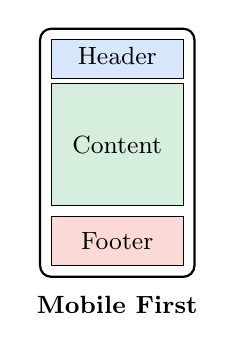
\begin{tikzpicture}[scale=0.7]
                \draw[rounded corners,thick] (0,0) rectangle (2.8,4.5);
                \draw[fill=googleblue!20] (0.2,3.6) rectangle (2.6,4.3);
                \node at (1.4,4) {\small Header};
                \draw[fill=googlegreen!20] (0.2,1.3) rectangle (2.6,3.5);
                \node at (1.4,2.4) {\small Content};
                \draw[fill=googlered!20] (0.2,0.2) rectangle (2.6,1.1);
                \node at (1.4,0.65) {\small Footer};
                \node at (1.4,-0.5) {\small\textbf{Mobile First}};
            \end{tikzpicture}
            \vspace{0.3cm}
            \begin{alertblock}{Accessibility}
                WCAG 2.1 compliant with voice support
            \end{alertblock}
        \end{center}
    \end{columns}
\end{frame}

% Creating technical architecture slide
\section{Architecture}
\begin{frame}{Technical Architecture}
    \begin{center}
        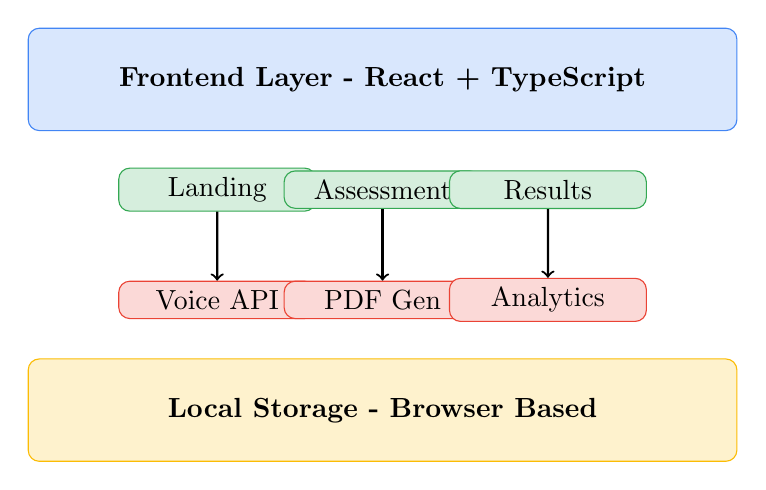
\begin{tikzpicture}[scale=0.7]
            \node[draw=googleblue,fill=googleblue!20,rounded corners,minimum width=9cm,minimum height=1.3cm] at (0,4) {\textbf{Frontend Layer - React + TypeScript}};
            
            \node[draw=googlegreen,fill=googlegreen!20,rounded corners,minimum width=2.5cm] (comp1) at (-3,2) {Landing};
            \node[draw=googlegreen,fill=googlegreen!20,rounded corners,minimum width=2.5cm] (comp2) at (0,2) {Assessment};
            \node[draw=googlegreen,fill=googlegreen!20,rounded corners,minimum width=2.5cm] (comp3) at (3,2) {Results};
            
            \node[draw=googlered,fill=googlered!20,rounded corners,minimum width=2.5cm] (serv1) at (-3,0) {Voice API};
            \node[draw=googlered,fill=googlered!20,rounded corners,minimum width=2.5cm] (serv2) at (0,0) {PDF Gen};
            \node[draw=googlered,fill=googlered!20,rounded corners,minimum width=2.5cm] (serv3) at (3,0) {Analytics};
            
            \node[draw=googleyellow,fill=googleyellow!20,rounded corners,minimum width=9cm,minimum height=1.3cm] at (0,-2) {\textbf{Local Storage - Browser Based}};
            
            \draw[->,thick] (comp1) -- (serv1);
            \draw[->,thick] (comp2) -- (serv2);
            \draw[->,thick] (comp3) -- (serv3);
        \end{tikzpicture}
    \end{center}
    
    \vspace{0.3cm}
    \begin{beamercolorbox}[wd=0.9\textwidth,sep=5pt,center,rounded=true]{palette secondary}
        \color{white}\textbf{Privacy First:} All data stored locally - No server uploads
    \end{beamercolorbox}
\end{frame}

% Creating future enhancements slide
\section{Future Roadmap}
\begin{frame}{Future Enhancements}
    \begin{columns}[T]
        \column{0.48\textwidth}
        \begin{block}{Planned Features}
            \begin{itemize}
                \item \textcolor{googleblue}{\faIcon{brain}} AI coaching
                \item \textcolor{googlegreen}{\faIcon{mobile}} Native mobile app
                \item \textcolor{googlered}{\faIcon{language}} Multi-language
                \item \textcolor{googleyellow}{\faIcon{chart-line}} Progress tracking
            \end{itemize}
        \end{block}
        
        \begin{block}{Integration Plans}
            \begin{itemize}
                \item Calendar sync
                \item Therapist network
                \item Video sessions
                \item Community forums
            \end{itemize}
        \end{block}
        
        \column{0.48\textwidth}
        \begin{center}
            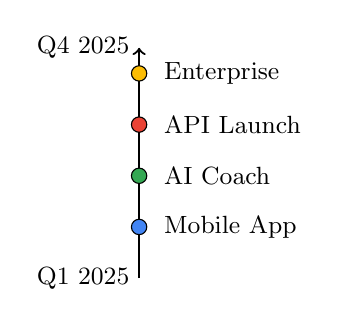
\begin{tikzpicture}[scale=0.65]
                \draw[thick,->] (0,0) -- (0,4.5);
                \node[left] at (0,0) {\small Q1 2025};
                \node[left] at (0,4.5) {\small Q4 2025};
                
                \draw[fill=googleblue] (0,1) circle (0.15cm);
                \node[right] at (0.3,1) {\small Mobile App};
                
                \draw[fill=googlegreen] (0,2) circle (0.15cm);
                \node[right] at (0.3,2) {\small AI Coach};
                
                \draw[fill=googlered] (0,3) circle (0.15cm);
                \node[right] at (0.3,3) {\small API Launch};
                
                \draw[fill=googleyellow] (0,4) circle (0.15cm);
                \node[right] at (0.3,4) {\small Enterprise};
            \end{tikzpicture}
            \vspace{0.3cm}
            \begin{alertblock}{Vision 2025}
                Become the leading AI-powered relationship assessment platform
            \end{alertblock}
        \end{center}
    \end{columns}
\end{frame}

% Creating demo screenshots slide
\section{Demo}
\begin{frame}{Live Demo Screenshots}
    \begin{center}
        \begin{tikzpicture}[scale=0.8]
            \node[draw,thick,minimum width=3.5cm,minimum height=2.8cm,fill=gray!10] at (0,0) {
                \begin{minipage}{3.2cm}
                    \centering
                    \textbf{Landing Page}\\
                    \vspace{0.4cm}
                    \faIcon{home} \\
                    \small Partner Selection\\
                    Assessment Types
                \end{minipage}
            };
            
            \node[draw,thick,minimum width=3.5cm,minimum height=2.8cm,fill=gray!10] at (4.5,0) {
                \begin{minipage}{3.2cm}
                    \centering
                    \textbf{Question Card}\\
                    \vspace{0.4cm}
                    \faIcon{question-circle} \\
                    \small Dual Rating\\
                    Progress Bar
                \end{minipage}
            };
            
            \node[draw,thick,minimum width=3.5cm,minimum height=2.8cm,fill=gray!10] at (9,0) {
                \begin{minipage}{3.2cm}
                    \centering
                    \textbf{Results Page}\\
                    \vspace{0.4cm}
                    \faIcon{chart-pie} \\
                    \small Compatibility\\
                    PDF Download
                \end{minipage}
            };
            
            \draw[->,thick,googleblue] (1.75,0) -- (2.75,0);
            \draw[->,thick,googlegreen] (6.25,0) -- (7.25,0);
        \end{tikzpicture}
    \end{center}
    
    \vspace{0.4cm}
    \begin{beamercolorbox}[wd=0.9\textwidth,sep=5pt,center,rounded=true,shadow=true]{palette primary}
        \color{white}\faIcon{globe} \textbf{Try it now:} \href{https://lovable.dev/projects/3acd99c3-d680-4dc3-bca4-795980f0aceb}{lovable.dev/projects/3acd99c3}
    \end{beamercolorbox}
\end{frame}

% Creating final slide
{
\setbeamertemplate{headline}{}
\setbeamertemplate{footline}{}
\begin{frame}
    \begin{tikzpicture}[remember picture,overlay]
        \fill[googleblue!15] (current page.south west) rectangle (current page.north east);
    \end{tikzpicture}
    
    \begin{center}
        {\Huge \color{googleblue}\textbf{Thank You!}}\\
        \vspace{0.4cm}
        {\LARGE \color{darkgray}Questions \& Discussion}\\
        
        \vspace{0.8cm}
        
        \begin{minipage}{0.7\textwidth}
            \centering
            \begin{beamercolorbox}[wd=\textwidth,sep=12pt,center,rounded=true,shadow=true]{palette primary}
                \color{white}
                \textbf{Connect With Us}\\
                \vspace{0.4cm}
                \faIcon{globe} \href{https://easy-ai-labs.lovable.app/}{\color{white}easy-ai-labs.lovable.app}\\
                \vspace{0.2cm}
                \faIcon{linkedin} \href{https://www.linkedin.com/in/yashkavaiya}{\color{white}linkedin.com/in/yashkavaiya}\\
                \vspace{0.2cm}
                \faIcon{building} \href{https://www.linkedin.com/company/genai-guru}{\color{white}Gen AI Guru}\\
                \vspace{0.2cm}
                \faIcon{youtube} \href{https://youtube.com/@genai-guru}{\color{white}YouTube: @genai-guru}
            \end{beamercolorbox}
        \end{minipage}
        
        \vspace{0.8cm}
        
        \begin{columns}[T]
            \column{0.33\textwidth}
            \begin{center}
                \textcolor{googlered}{\Large\faIcon{heart}}\\
                \small\textbf{86 Questions}
            \end{center}
            
            \column{0.33\textwidth}
            \begin{center}
                \textcolor{googlegreen}{\Large\faIcon{users}}\\
                \small\textbf{14 Categories}
            \end{center}
            
            \column{0.33\textwidth}
            \begin{center}
                \textcolor{googleyellow}{\Large\faIcon{star}}\\
                \small\textbf{AI Powered}
            \end{center}
        \end{columns}
        
        \vspace{0.6cm}
        {\small\color{darkgray}\textit{Follow for more AI innovations in relationship technology}}
    \end{center}
\end{frame}
}

\end{document}
